A view is a SELECTION of columns from one or more tables.  It is a {\textquotedbl}virtual{\textquotedbl} table, you can see and process the information, but ``virtual'' means that the view table does not physically exist.  The rows appearing in the view are derived from underlying base tables.  Changes in the base tables are reflected directly in the views.  Views are part of the external user schema and enable a high degree of logical data independence.

\ \ CREATE VIEW view\_name ( col\_name1 [ , col\_name2 ... ] )

\ \ AS 

\ \ SELECT ...

For example:

\ \ CREATE VIEW EMP\_VIEW

\ \ \ \ (EMPLOYEE\_NO, NAME, DEPARTMENT)

\ \ AS

\ \ \ \ SELECT\ \ E.EMPNO, E.ENAME, D.DNAME

\ \ \ \ FROM\ \ \ \ EMP E

\ \ \ \ INNER JOIN\ \ DEPT D

\ \ \ \ \ \ ON\ \ E.DEPTNO = D.DEPTNO;



\begin{center}
  
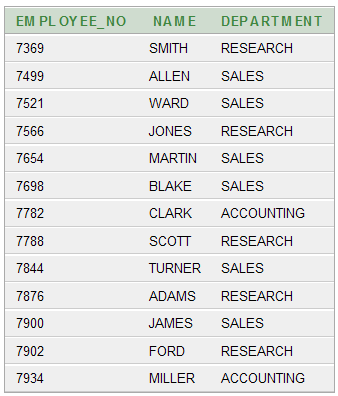
\includegraphics[width=9.063cm,height=10.472cm]{images/img (50).png}

\end{center}
We then use the view as if it was a table:

\ \ SELECT * FROM EMP\_VIEW;

Views are useful for:

\begin{itemize}
\item Restricting access to the database to only the data users need to access;
\item Providing a simple table for users in place of asking them to use a complex queries
\item Providing data independence for users, that is making sure that the data remains available for them, through up to date views, even though the underlying  data structure changes..
\end{itemize}
This view provides staff and department information without having to perform the join each time the request has to be met.  Select queries may now be run against this view as though it were a single table in the database.  Updates on the staff using this view will be stored in the base table, EMP, and updates on departments using this view will be stored in the base table, DEPT.

H1\ \ Create a view called CUSTOMER which contains customer name, address and area.

\begin{flushleft}
\tablefirsthead{}
\tablehead{}
\tabletail{}
\tablelasttail{}
\begin{supertabular}{|m{14.303cm}|}
\hline
CREATE

\\\hline
\end{supertabular}
\end{flushleft}
\ \ Can the table CUST be updated using this view?

H2\ \ Create a view called ACCOUNT\_BALANCE which contains customer reference number, account number and balance.

\begin{flushleft}
\tablefirsthead{}
\tablehead{}
\tabletail{}
\tablelasttail{}
\begin{supertabular}{|m{14.583cm}|}
\hline
CREATE

\\\hline
\end{supertabular}
\end{flushleft}
\ \ Can the tables CUST or ACC be updated through this view?

H3\ \ Based on view H2 and another table, create a view to display details of customers, who have balances greater than £500.

\begin{flushleft}
\tablefirsthead{}
\tablehead{}
\tabletail{}
\tablelasttail{}
\begin{supertabular}{|m{14.583cm}|}
\hline
CREATE

\\\hline
\end{supertabular}
\end{flushleft}
SUBQUERIES

If we take an example such as to find out which account(s) has the largest balance, thinking about this question logically, it falls into 2 parts.  

Firstly we need to find out what the largest balance is:



\begin{center}
  
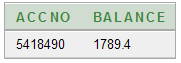
\includegraphics[width=1.819cm,height=0.871cm]{images/img (51).png}

\end{center}
\ \ SELECT MAX(BALANCE) FROM ACC

secondly we need to find which account(s) this is against.

SQL supports this strategy for querying the database through the use of subqueries.  The subquery is processed first; the result of the subquery is then substituted into the WHERE clause of the outer query.

\ \ SELECT \ \ ACCNO, BALANCE

\ \ FROM \ \ ACC

\ \ WHERE \ \ BALANCE = 

\ \ \ \ \ \ \ \ (SELECT MAX(BALANCE) FROM ACC) ;

Care needs to be taken with the WHERE clause.  In this example the inner statement (subquery) returns a single value (£1,789.40), so the subquery condition will work:



\begin{center}
  
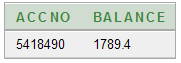
\includegraphics[width=4.819cm,height=1.669cm]{images/img (51).png}

\end{center}
If the inner SELECT can return several rows then the condition would need to take this into account e.g. WHERE column IN (SELECT{\dots}..).

\ \ SELECT \ \ ACCNO, BALANCE

\ \ FROM \ \ ACC

\ \ WHERE \ \ BRANCH IN 

\ \ \ \ \ \ \ \ (SELECT DISTINCT BRANCH FROM ACC) ;

H4\ \ In this example, the where clause is not adding anything to this last query. Why is that?

\begin{flushleft}
\tablefirsthead{}
\tablehead{}
\tabletail{}
\tablelasttail{}
\begin{supertabular}{|m{14.583cm}|}
\hline
\\\hline
\end{supertabular}
\end{flushleft}
Remember, the subquery is a complete query in its own right, it should be written first, run and checked, and only then incorporated into the full query.

\begin{center}
  

\includegraphics[width=1.048cm,height=0.903cm]{images/img (2).png}

\end{center}
H5\ \ Who has the highest basic salary?

This cannot be answered straight off - try finding the answer by looking at the printed tables from the Personnel System.  Firstly, we need to know what is the highest salary (and that can be only one value) before we can decide who has that salary - and there may be more than one employee with that salary.

What is the highest salary?

Select

From\ \ \ \ \ \ \ \ \ \ \ \ \ \   

;

Run the query.  How many results are displayed?  There should be only one!

Now place that Select statement as the sub-query (enclosed in brackets and without the semi-colon) and determine who has that salary.

\begin{flushleft}
\tablefirsthead{}
\tablehead{}
\tabletail{}
\tablelasttail{}
\begin{supertabular}{|m{14.551001cm}|}
\hline
Select

From

Where

\ \ \ \ = (Select  This is the subquery

\ \ \ \   From\ \ \ \ \ \   ) ;\ \   from above

\\\hline
\end{supertabular}
\end{flushleft}
H6 \ \ Which salesman earns the most, including commission?

Hint - Create and check a query to determine the highest income (salary + commission) for salesmen, and then determine which salesmen earn that income by using that query as the subquery.

\begin{flushleft}
\tablefirsthead{}
\tablehead{}
\tabletail{}
\tablelasttail{}
\begin{supertabular}{|m{14.551001cm}|}
\hline
Select

From

Where

And\ \ \ \ \ \ 

\ \ \ \ \ \ = (Select

\ \ \ \ \ \   From

\ \ \ \ \ \   Where\ \ \ \ \ \ \ \ \ \ ) ;

\\\hline
\end{supertabular}
\end{flushleft}
\ \ Is CLARKE one of the displayed employees?  He is a MANAGER!

H6\ \ Who in New York has the highest income (salary + commission)?  Don't work out who works in department 10, department codes may change next week!

What has to be determined before the main results can be selected?

Carefully check the results of your answer against the original tables.

\begin{flushleft}
\tablefirsthead{}
\tablehead{}
\tabletail{}
\tablelasttail{}
\begin{supertabular}{|m{14.551001cm}|}
\hline
Select

From

INNER Join  

ON

Where

And\ \ \ \ \ \ 

\ \ \ \ \ \ =(Select

\ \ \ \ \ \   From

\ \ \ \ \ \   INNER Join  

\ \ \ \ \ \   ON

\ \ \ \  \ \   Where\ \ \ \ \ \ \ \   );\\\hline
\end{supertabular}
\end{flushleft}
H7 \ \ List the names of the people who work in the same department as Jones (you may use the fact that his Employee number is 7566 as there may be more than one 'JONES' on the list)

\begin{flushleft}
\tablefirsthead{}
\tablehead{}
\tabletail{}
\tablelasttail{}
\begin{supertabular}{|m{14.551001cm}|}
\hline
Select

From

Where

And

\ \ \ \ \ \ =(Select

\ \ \ \ \ \   From

\ \ \ \ \ \   Where \ \ \ \ \ \ \ \ \ \ );\\\hline
\end{supertabular}
\end{flushleft}
Have you displayed 5 employees?  Have you displayed JONES?  If so, does JONES really work with himself?

H8\ \ List the names of anyone who started work on the same date as FORD.

\begin{flushleft}
\tablefirsthead{}
\tablehead{}
\tabletail{}
\tablelasttail{}
\begin{supertabular}{|m{14.551001cm}|}
\hline
Select

\\\hline
\end{supertabular}
\end{flushleft}
H9\ \ Does anyone have a basic salary that is the same as that of FORD ?

\begin{flushleft}
\tablefirsthead{}
\tablehead{}
\tabletail{}
\tablelasttail{}
\begin{supertabular}{|m{14.551001cm}|}
\hline
Select

\\\hline
\end{supertabular}
\end{flushleft}
H10\ \ What is the average salary of those employees on Grade 2?  Use a subquery \ \ in your solution.

\begin{flushleft}
\tablefirsthead{}
\tablehead{}
\tabletail{}
\tablelasttail{}
\begin{supertabular}{|m{14.551001cm}|}
\hline
Select

\\\hline
\end{supertabular}
\end{flushleft}
Now produce a solution without using a subquery.

\begin{flushleft}
\tablefirsthead{}
\tablehead{}
\tabletail{}
\tablelasttail{}
\begin{supertabular}{|m{14.551001cm}|}
\hline
Select

\\\hline
\end{supertabular}
\end{flushleft}
H11 \ \ Find the name and salary of the people who earn more than the average salary of those on grade 2.

\begin{flushleft}
\tablefirsthead{}
\tablehead{}
\tabletail{}
\tablelasttail{}
\begin{supertabular}{|m{14.551001cm}|}
\hline
Select

\\\hline
\end{supertabular}
\end{flushleft}

\clearpage
